
\Problem{Arbres --- Recorreguts recursius}

\Statement

Feu un programa que llegeixi la descripció d'un arbre binari de naturals
i escrigui els seus recorreguts en postordre i inordre.

\medskip

La descripció d'un arbre
consisteix en el seu recorregut en preordre,
el qual inclou les fulles marcades amb un -1.

\medskip


Per exemple, l'arbre

\begin{center}
\begin{latexonly}
  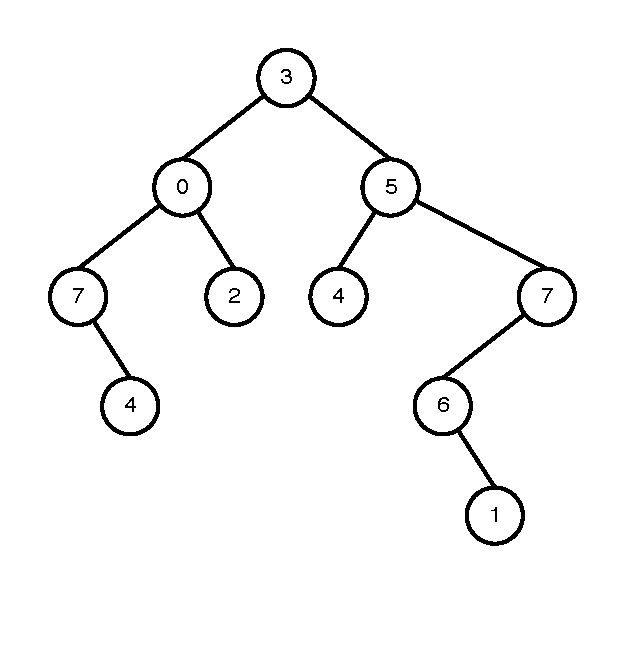
\includegraphics[height=6cm]{tree.pdf}
\end{latexonly}
\begin{htmlonly}
  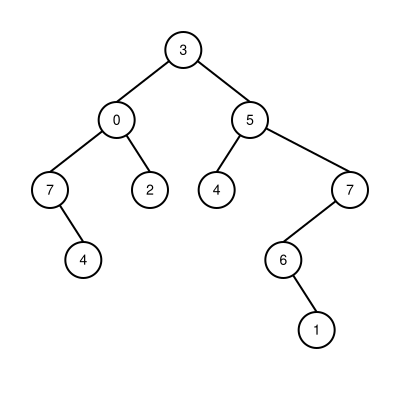
\includegraphics[height=6cm]{tree.svg}
\end{htmlonly}
\end{center}

es descriuria amb
{\tt \small
\quad 3 0 7 -1 4 -1 -1 2 -1 -1 5 4 -1 -1 7 6 -1 1 -1 -1 -1
\normalsize
}

\Input

L'entrada consisteix en la descripció d'un arbre binari de naturals.

\Output

Escriviu dues línies, amb els recorreguts en postordre i inordre de l'arbre.
Seguiu el format de l'exemple.



\SampleOneCol
